\documentclass[twoside]{article}
\input{ISC18-english.sty}
%%%%%%%%%%%%%%%%%%%%%%%%%%%%  Make sure to compile twice for proper cross-references. %%%%%%%%%%%%%%%%%%%%%%%
%%%%%%% For proper display of references, compile the document twice. %%%%%%%%%%%%%%%%%%%%% 
%%%%%%%%%%%%%%% If using TeX Live, compile using pdflatex command %%%%%%%%%%%%%%%%%%%%%%%
\begin{document}
\thispagestyle{empty}
%%%%%%%%%%%%%%%%% Article title header  %%%%%%%%%%%%%%%%%%%%
\fancyhead[LE]{Extropy of the Residual Lifetime}
%%%%%%%%%%%%%%%%% Article authors header   %%%%%%%%%%%%%%%%%%%%
\fancyhead[RO]{
Z. Pakdaman and R. Alizadeh Noughabi
}
\begin{center}
{
\includegraphics [height=25mm, width=150.3mm] {Images/isc18E}} \\
\vspace*{-1.8cm}
%\begin{center}
%\color{blue} 
%{\hspace{0.1cm}\rule{\textwidth}{1mm}}\\
%\end{center}
\vspace*{4cm}
%%%%%%%%%%%%%%%%% Article title  %%%%%%%%%%%%%%%%%%%%
{\Large \bf  Extropy of the Residual Lifetime of Alive Components in Coherent Systems}\\
%%%%%%%%%%%%%%%%% Article authors and affiliations %%%%%%%%%%%%%%%%%%%%
{\bf
Zohreh Pakdaman$^1$, Reza Alizadeh Noughabi  \footnote{{\bf Corresponding Author:} {\tt zpakdaman@hormozgan.ac.ir }} \\
$^1$Department of Statistics, University of Hormozgan, Hormozgan,  Iran}
\end{center}
\rule{\textwidth}{0.2mm}\\
%%%%%%%%%%%%%%%%% Article abstract  %%%%%%%%%%%%%%%%%%%%
\noindent{\bf Abstract:}\\
This research investigates the uncertainty associated with the remaining lifetimes of alive components in coherent systems after system failure. Although the system may no longer function, some components may still remain alive, and the uncertainty in their remaining lifetimes can be meaningfully quantified. To this end, we employ extropy as a measure of uncertainty for the remaining lifetimes of alive components. By combining the system signature with conditional properties of order statistics, we develop a mathematical framework for this purpose. Focusing on the heavy-tailed Lomax distribution, our results provide insight into how the system structure affects the uncertainty of the remaining lifetimes of alive components after system failure.
 
\noindent{\bf Keywords:} 
Extropy, Coherent System,  Order statistics, System signature, Residual lifetimes of live components. \\
\noindent{\bf Mathematics Subject Classification (2010):} $62N05$;
$62F10$. \\
\hspace{1cm}\rule{\textwidth}{0.2mm}\\
%%%%%%%%%%%%%%
\section{Introduction}

The reliability analysis of coherent systems has traditionally prioritized the residual lifetime of alive components. However, contemporary risk assessment and maintenance engineering require a focus on the post-failure dynamics of individual units. When a system ceases to function at time $t$, specific units referred to herein as alive components may still exist with significant functional capacity. A critical objective in this context is the characterization of the residual lifetime of alive components, as this metric offers deep insights into structural safety and forensic reliability. Quantifying the uncertainty inherent in the residual lifetime of alive components is not merely a theoretical exercise; it serves as a prerequisite for developing optimized salvage strategies, predictive maintenance, and strategic resource allocation in complex systems.

The structural dependency of the system is characterized by its signature $\boldsymbol{s} = (s_1, \ldots, s_n)$, where $s_i = P(T(n) = Y_{i:n})$ represents the probability that the $i$-th component failure coincides with system failure \cite{Samaniego:2007}. This vector satisfies $\sum_{i=1}^{n} s_i = 1$ and provides a purely structural description of the system's reliability. In this paper, we specifically analyze coherent systems initiated at $t=0$ whose signature vector takes the following restricted form:
\begin{equation}
\boldsymbol s = (s_1, \ldots, s_i, 0, \ldots, 0), \qquad i = 1, \ldots, n-1.
\end{equation}
This formulation implies that system failure must occur by the $i$-th component failure at the latest. Consequently, at the moment of system collapse, any component $j > i$ is guaranteed to be an alive component. Building upon this framework, \cite{GoliforushaniAsadiBalakrishnan:2012} introduced a comprehensive mixture model to characterize the residual lifetime of alive components. This model provides the probabilistic foundation for evaluating the residual lifetime of alive components of the $j$-th ordered component, given that the system failure occurred prior to time $t$. To analyze the information-theoretic properties (such as extropy) of these alive components, we define the structural and stochastic components of the model one by one:

\begin{itemize}
    \item \textbf{The Residual Lifetime Variable ($T_{j,n}(t)$):} For $t>0$ and $j=i+1, \ldots, n$, this variable represents the residual lifetime of alive components beyond $t$, given the system failure before $t$ but the alive component remained:
    \begin{equation}
    T_{j,n}(t) = [Y_{j:n} - t \mid T(n) < t < Y_{j:n}].
    \end{equation}

    \item \textbf{Dynamic Component Weights ($p_k(t)$):} These weights represent the conditional probability that the system's failure was caused by the $k$-th component, given the system state at time $t$. Incorporating the system signature, they are defined as:
    \begin{equation}\label{pk}
    p_k(t) = P(T(n) = Y_{k:n} \mid T(n) < t < Y_{j:n}) = \frac{s_k [ \bar{G}_{Y_{k:n}}(t) - \bar{G}_{Y_{j:n}}(t) ] }{ \sum_{m=1}^i s_m [ \bar{G}_{Y_{m:n}}(t) - \bar{G}_{Y_{j:n}}(t) ] }.
    \end{equation}

    \item \textbf{State-Specific Coefficient ($K_{l,j,k,n}(t)$):} This accounts for the exact state of the system at time $t$, quantifying the probability that $l$ components are no longer functional, given a failure rank $k$ and the presence of the $j$-th alive component:
    \begin{equation}\label{kl}
    K_{l,j,k,n}(t) = \frac{ \bar{G}_{Y_{l+1:n}}(t) - \bar{G}_{Y_{l:n}}(t) }
    { \bar{G}_{Y_{j:n}}(t) - \bar{G}_{Y_{k:n}}(t)}.
    \end{equation}

    \item \textbf{Survival Function of Alive Components ($\bar{G}_{Y^t_{j-1:n-l}}(y)$):} This term represents the SF of the residual lifetime of alive components within a sub-sample of $n-l$ components, all aged by time $t$. \cite{GoliforushaniAsadiBalakrishnan:2012} derived this through the binomial expansion:
    \begin{equation}\label{eq_binom_sum}
    \bar{G}_{Y^t_{j-1:n-l}}(y) = \sum\limits_{m=n-j+1}^{n-l} \binom{n-l}{m} \left( \frac{\bar{G}(y+t)}{\bar{G}(t)} \right)^{m} \left( 1 - \frac{\bar{G}(y+t)}{\bar{G}(t)} \right)^{n-l-m}.
    \end{equation}
    Utilizing the relationship between binomial sums and the incomplete beta integral, this is represented as:
    \begin{equation}\label{eq_beta_int}
    \bar{G}_{Y^t_{j-1:n-l}}(y) = 1-(j-l)\binom{n-l}{n-j}\int_{\frac{\bar{G}(y+t)}{\bar{G}(t)}}^{1}u^{n-j}(1-u)^{j-l-1}~du.
    \end{equation}
\end{itemize}
By synthesizing these elements, the unified survival function for the residual lifetime of alive components is:
\begin{equation}\label{SF_Main}
\bar{G}_{T_{j,n}(t)}(y) = \sum\limits_{k=1}^{i} \sum\limits_{l=k}^{j-1} p_k(t) K_{l,j,k,n}(t) \bar{G}_{Y^t_{j-1:n-l}}(y).
\end{equation}
The probability density function (PDF) of the residual lifetime of an alive component, denoted by $g_{T_{j,n}(t)}(y)$, is obtained by taking the negative derivative of the survival function in \eqref{SF_Main} with respect to $y$. This results in the following mixture model:
\begin{equation}\label{PDF_Main}
g_{T_{j,n}(t)}(y) = \sum\limits_{k=1}^{i} \sum\limits_{l=k}^{j-1} p_k(t) K_{l,j,k,n}(t) g_{Y^t_{j-1:n-l}}(y),
\end{equation}
where $g_{Y^t_{j-1:n-l}}(y)$ is the PDF of the $(j-l)$-th order statistic among $n-l$ aged survivors, all of which have exceeded age $t$. Based on the structural properties of order statistics, this density can be expressed as:
\begin{equation}
g_{Y^t_{j-1:n-l}}(y) = \frac{(n-l)!}{(j-l-1)!(n-j)!} \frac{g(y+t)}{\bar{G}(t)} \left[ \frac{\bar{G}(y+t)}{\bar{G}(t)} \right]^{n-j} \left[ 1 - \frac{\bar{G}(y+t)}{\bar{G}(t)} \right]^{j-l-1}.
\end{equation}
In this framework, the PDF $g_{T_{j,n}(t)}(y)$ characterizes the instantaneous failure rate of the alive component at time $y+t$, conditioned on the system having failed at time $t$ while the $j$-th component was still alive.
%A substantial body of research has examined the residual lifetimes of coherent systems under a variety of reliability settings and modeling frameworks; see, for instance, \cite{Samaniego1985}, \cite{KocharMukerjeeSamaniego1999}, \cite{BairamovAhsanullahAkhundov2002}, \cite{KhalediShaked2007}, \cite{AsadiGoliforushani2008}, and \cite{Zhang2025}. These studies collectively highlight the central role of residual lifetime analysis in understanding the post-failure behavior of coherent structures and in developing refined probabilistic descriptions of surviving components.

In reliability analysis, uncertainty is traditionally measured by Shannon entropy \cite{Shannon:1948}, defined for a continuous random variable $X$ as $H(X)=-E\{\log f(X)\}$. However, a compelling alternative is \emph{extropy}, a dual concept to entropy that emphasizes density concentration.
 For a non-negative variable $X$, extropy is given by:
\begin{equation*}\label{eq:extropy_def}
J(X) = -\frac{1}{2}\int_{0}^{+\infty} f^{2}(x)\,dx = -\frac{1}{2}\int_{0}^{1} f\big(F^{-1}(u)\big)\,du.
\end{equation*}
While entropy captures average unpredictability, extropy is more sensitive to the distributional structure, making it highly effective for studying survival data. Recent advancements by Pakdaman and colleagues have significantly expanded this field, investigating extropy in the context of dynamic uncertainty, stochastic ageing, and system reliability \cite{ PakdamanNoughabi:2025b, PakdamanAlizadehNoughabi:2025c, PakdamanNoughabi:2026}. Following this informational perspective, we apply extropy to evaluate the residual lifetime of alive components in coherent systems.
 Equation \eqref{SF_Main} constitutes the foundational mathematical representation for all subsequent extropy calculations in this study. Extropy provides a unique measure of "order" and predictability, making it ideal for assessing the residual lifetime of alive components in post-failure scenarios. In the following sections, we utilize this framework to derive closed-form expressions for extropy, establish stochastic bounds, and investigate the behavior of alive components under the Lomax distribution.
 
 The rest of this paper is organized as follows. In Section 2, we study the extropy associated with the residual lifetimes of components that continue to operate after the failure of a coherent system. By using the system signature and conditional properties of order statistics, an explicit expression for the proposed extropy measure is derived. Moreover, a lower bound for this measure is established. Finally, Section 3 presents the concluding remarks and summarizes the main findings of the paper.

%%%%%%%%%%%%%%%%%%%%%%% Definition %%%%%%%%%%%%%%%%%%%%%%%%%%%%%%%%%
\section{Extropy Analysis of the Residual Lifetime of Alive Components}

Based on the density function of the residual lifetime of an alive component given in \eqref{PDF_Main}, the extropy of $T_{j,n}(t)$ is defined by
\begin{equation}\label{Extropy_Def_Tjn}
J\left(T_{j,n}(t)\right)
=
-\frac{1}{2}
\int_{0}^{\infty}
g_{T_{j,n}(t)}^{2}(y)\,dy .
\end{equation}

Substituting the mixture density in \eqref{PDF_Main} into \eqref{Extropy_Def_Tjn}, we obtain
\begin{equation}\label{Extropy_Mixture_Form}
J\left(T_{j,n}(t)\right)
=
-\frac{1}{2}
\int_{0}^{\infty}
\left[
\sum_{k=1}^{i}
\sum_{l=k}^{j-1}
p_k(t)K_{l,j,k,n}(t)
g_{Y^t_{j-1:n-l}}(y)
\right]^2
dy .
\end{equation}

Now, using \eqref{pk} and \eqref{kl}, the product $p_k(t)K_{l,j,k,n}(t)$ is simplified as
\begin{equation}\label{Product_pk_K}
p_k(t)K_{l,j,k,n}(t)
=
\frac{
s_k\left[
\bar{G}_{Y_{l+1:n}}(t)
-
\bar{G}_{Y_{l:n}}(t)
\right]
}{
\sum\limits_{m=1}^{i}
s_m\left[
\bar{G}_{Y_{j:n}}(t)
-
\bar{G}_{Y_{m:n}}(t)
\right]
}.
\end{equation}

Therefore, by substituting the product \eqref{Product_pk_K} into \eqref{Extropy_Mixture_Form}, we obtain
\begin{equation}\label{Extropy_After_Product}
J\left(T_{j,n}(t)\right)
=
-\frac{1}{2}
\int_{0}^{\infty}
\left[
\frac{
\sum\limits_{k=1}^{i}
\sum\limits_{l=k}^{j-1}
s_k
\left[
\bar{G}_{Y_{l+1:n}}(t)
-
\bar{G}_{Y_{l:n}}(t)
\right]
g_{Y^t_{j-1:n-l}}(y)
}{
\sum\limits_{m=1}^{i}
s_m
\left[
\bar{G}_{Y_{j:n}}(t)
-
\bar{G}_{Y_{m:n}}(t)
\right]
}
\right]^2
dy .
\end{equation}

Finally, under the transformation
$
u=\frac{\bar{G}(y+t)}{\bar{G}(t)},
$
the extropy can be expressed as
\begin{equation}\label{Extropy_Final}
J\left(T_{j,n}(t)\right)
=
-\frac{1}{2}
\int_{0}^{1}
\left[
\frac{
\sum\limits_{k=1}^{i}
\sum\limits_{l=k}^{j-1}
s_k
\left[
\bar{G}_{Y_{l+1:n}}(t)
-
\bar{G}_{Y_{l:n}}(t)
\right]
\beta_{l,j,n}(u)
}{
\sum\limits_{m=1}^{i}
s_m
\left[
\bar{G}_{Y_{j:n}}(t)
-
\bar{G}_{Y_{m:n}}(t)
\right]
}
\right]^2
\frac{
g\left(G^{-1}\left(\bar{G}(t)u\right)\right)
}{
\bar{G}(t)
}
\,du ,
\end{equation}
where
\begin{equation}\label{beta_def}
\beta_{l,j,n}(u)
=
(j-l)\binom{n-l}{n-j}
u^{\,n-j}(1-u)^{\,j-l-1},
\qquad 0<u<1.
\end{equation}

Here, $\beta_{l,j,n}(u)$ is the kernel associated with the density of the relevant order statistic after the above transformation. Hence, formula \eqref{Extropy_Final} follows directly from substituting the simplified product $p_k(t)K_{l,j,k,n}(t)$ into the extropy integral and then rewriting the density term in terms of $\beta_{l,j,n}(u)$.
This expression provides a comprehensive basis for analyzing how the uncertainty of the residual lifetime of an alive component evolves relative to the system's age $t$. The integral effectively captures the interplay between the system's topological configuration (via the signature) and the underlying ageing characteristics of the components.




\begin{eg}
Consider a coherent system with \(n=5\), \(i=3\), and \(j=4\), and suppose that its signature is
$
\boldsymbol{s}=(0.20,\,0.50,\,0.30,\,0,\,0).
$
Assume that the component lifetimes follow the Lomax distribution with distribution function, survival function, and density
$
G(x)=1-\left(1+\frac{x}{\lambda}\right)^{-\alpha}, ~
\bar G(x)=\left(1+\frac{x}{\lambda}\right)^{-\alpha}, ~
g(x)=\frac{\alpha}{\lambda}\left(1+\frac{x}{\lambda}\right)^{-(\alpha+1)},
$
for \(x>0\), \(\alpha>0\), and \(\lambda>0\).
Using the exact numerical representation
$
J(T_{4,5}(t))
=
-\frac12\int_0^\infty g_{T_{4,5}(t)}^2(y)\,dy,
$
where \(g_{T_{4,5}(t)}\) is obtained from the mixture representation derived in \eqref{Extropy_Final}, we evaluate numerically the extropy of the residual lifetime of alive components for different values of the Lomax parameters. In the left panel of Figure~\ref{fig:lomax-extropy}, \(\lambda=1\) is fixed and \(\alpha\) varies over
$
0.8,\ 1.8,\ 2.4,\ 3.
$
In the right panel, \(\alpha=2\) is fixed and \(\lambda\) varies over
$
0.6,\ 1,\ 1.4,\ 1.8.
$
In both panels, the extropy is plotted for \(0.1\le t\le 1.5\).
\begin{figure}[ht]
\begin{center}
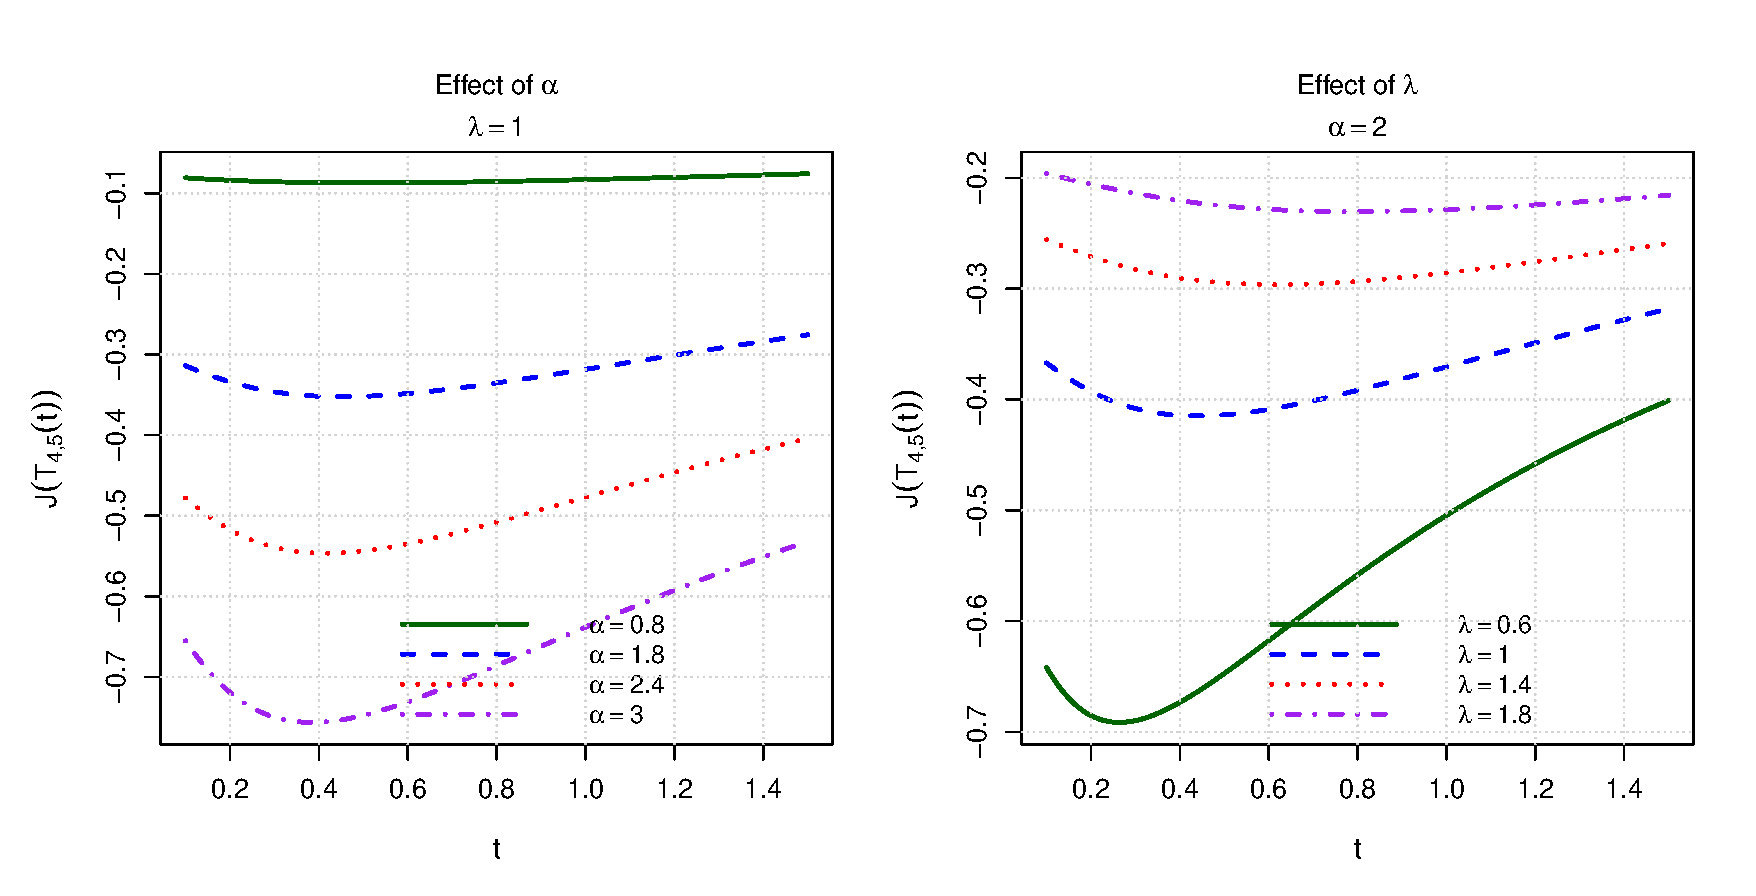
\includegraphics[width=13cm,height=6cm]{Images/example1.eps}\\
\vspace{-0.2cm}
\caption{\footnotesize{Extropy of the lifetimes of components that continue to operate after system failure, \(J(T_{4,5}(t))\), for a coherent system with signature \(\boldsymbol{s}=(0.20,0.50,0.30,0,0)\) under the Lomax model. Left panel: effect of \(\alpha\) with \(\lambda=1\). Right panel: effect of \(\lambda\) with \(\alpha=2\).}}
\label{fig:lomax-extropy}
\end{center}
\end{figure}
Figure~\ref{fig:lomax-extropy} shows that \(J(T_{4,5}(t))\) is negative for all values of \(t\) and for all selected parameter combinations. Since more negative values of extropy correspond to greater uncertainty, lower curves indicate a higher uncertainty in the residual lifetime of alive components.
In both panels, the curves are non-monotone in \(t\). For each parameter combination, the extropy first decreases, reaches a minimum at an intermediate age, and then increases. Hence, the uncertainty first increases and then decreases over time, attaining its highest level at some intermediate ages.
The left panel shows the effect of the shape parameter \(\alpha\) when \(\lambda=1\). For each fixed \(t\), larger values of \(\alpha\) lead to more negative values of \(J(T_{4,5}(t))\), and therefore to greater uncertainty. In particular, the curve for \(\alpha=3\) is the lowest, whereas the curve for \(\alpha=0.8\) is the highest.
The right panel illustrates the effect of the scale parameter \(\lambda\) when \(\alpha=2\). For each fixed \(t\), larger values of \(\lambda\) produce less negative values of \(J(T_{4,5}(t))\), which indicates lower uncertainty. Thus, among the selected values, \(\lambda=0.6\) gives the greatest uncertainty, while \(\lambda=1.8\) gives the smallest.
Although the hazard rate of the Lomax distribution,
$
h(t)=\frac{\alpha}{\lambda+t},
$
is decreasing in \(t\), the uncertainty measured by extropy is not monotone in \(t\). Therefore, the behavior of the residual lifetime uncertainty cannot be explained solely by the monotonicity of the hazard rate and should be interpreted through the full conditional distribution.
Overall, Figure~\ref{fig:lomax-extropy} indicates that larger values of \(\alpha\) increase uncertainty, whereas larger values of \(\lambda\) decrease uncertainty. Moreover, the effect of age \(t\) is non-monotone: the uncertainty first increases and then decreases.
\end{eg}

Since the exact computation of the extropy of the residual lifetime of alive components may be difficult in practice, the following result provides a convenient lower bound.

\begin{thm}\label{th1}
Let $T_{j,n}(t)$ denote the residual lifetime of alive components in a coherent system. Then
\begin{equation}
J(T_{j,n}(t)) \geq \sum_{k=1}^{i}\sum_{l=k}^{j-1} p_k(t)\,K_{l,j,k,n}(t)\,J\!\left(Y^t_{j-l:n-l}\right).
\end{equation}
\end{thm}
\begin{proof}
The proof follows directly from the mixture representation in \eqref{PDF_Main} and the definition of extropy in \eqref{Extropy_Def_Tjn}. 
In particular, using Jensen's inequality for the convex function \(u^2\), together with the nonnegativity of the weights \(p_k(t)\) and \(K_{l,j,k,n}(t)\) given in \eqref{pk} and \eqref{kl}, yields the stated lower bound immediately.
\end{proof}


\begin{eg}
Consider a coherent system with \(n=5\), \(i=3\), and \(j=4\), whose signature vector is
$
\boldsymbol{s}=(0.20,\,0.50,\,0.30,\,0,\,0).
$
Assume that the component lifetimes follow the Lomax model considered in the previous example, with parameter values
$
\alpha=2
~ \text{and} ~
\lambda=1.
$
To illustrate the lower bound obtained in Theorem~\ref{th1}, we numerically compute both the exact extropy \(J(T_{4,5}(t))\) and its lower bound over the interval
$
0.1 \le t \le 1.5.
$
Figure~\ref{fig:lomax-lower-bound} displays the exact extropy curve together with the corresponding lower-bound curve. It is seen that, for all values of \(t\) in the plotted interval, the lower bound remains below the exact extropy. Hence, the numerical results confirm the validity of the inequality stated in Theorem~\ref{th1}.
\begin{figure}[ht]
\begin{center}
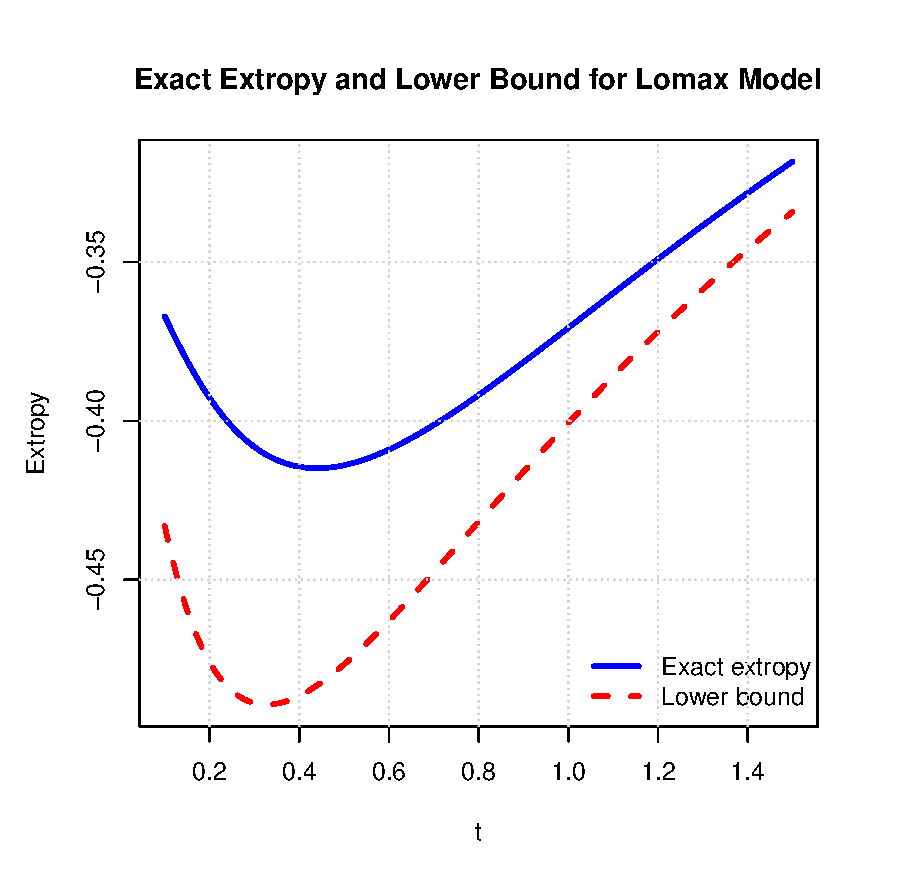
\includegraphics[width=7cm,height=6cm]{Images/example2.eps}\\
\vspace{-0.2cm}
\caption{\footnotesize{Exact extropy \(J(T_{4,5}(t))\) and its lower bound for a coherent system with signature \(\boldsymbol{s}=(0.20,0.50,0.30,0,0)\) under the Lomax model with \(\alpha=2\) and \(\lambda=1\).}}
\label{fig:lomax-lower-bound}
\end{center}
\end{figure}
The figure also shows that both curves have the same general shape. In particular, they are non-monotone in \(t\): each curve first decreases, reaches a minimum at an intermediate value of \(t\), and then increases. Therefore, the lower bound not only satisfies the theoretical inequality, but also captures the main qualitative behavior of the exact extropy.
Overall, this example provides a numerical verification of Theorem~\ref{th1}. The lower-bound curve consistently stays below the exact extropy curve over the whole interval \(0.1 \le t \le 1.5\), and thus the theoretical result is clearly confirmed.
\end{eg}


\section{Conclusion}

In this paper, we studied the extropy of the residual lifetime of alive components in coherent systems using the system signature and conditional order statistics. 
An explicit mixture representation was used to derive the extropy of \(T_{j,n}(t)\) and to describe the effect of the system structure on the uncertainty of surviving components. 
For Lomax-distributed component lifetimes, the numerical results showed that the extropy is non-monotone in the system age \(t\). 
It was also observed that larger values of \(\alpha\) increase uncertainty, whereas larger values of \(\lambda\) reduce it. 
Finally, a lower bound for the extropy was established and numerically verified, confirming its consistency with the exact extropy curve.
 %%%%%%%%%%%%%%%%%%%%%%%%%%%%%%%%%

%%%%%%%%%%%%%%%%%%%%%%%% References %%%%%%%%%%%%%%%%%%%%%%%%%%%%%

\begin{thebibliography}{9}
\bibitem[Samaniego (2007)]{Samaniego:2007}
Samaniego, F. J. (2007). {\it System Signatures and Their Applications in Engineering Reliability}, Springer, New York.

\bibitem[Goliforushani et al. (2012)]{GoliforushaniAsadiBalakrishnan:2012}
Goliforushani, S., Asadi, M. and Balakrishnan, N. (2012), On the residual and inactivity times of the components of used coherent systems, {\it Journal of Applied Probability},  49(2), 385-404.


\bibitem[Shannon (1948)]{Shannon:1948}
Shannon, C. (1948). A mathematical theory of communication, {\it The Bell System Technical Journal},  27(3), 379-423.

\bibitem[Pakdaman and Noughabi (2025b)]{PakdamanNoughabi:2025b}
Pakdaman, Z. and Noughabi, R. A. (2025b), On the study of the cumulative residual extropy of mixed used systems and their complexity, {\it Probability in the Engineering and Informational Sciences},  39(1), 122-140.

\bibitem[Pakdaman  Alizadeh Noughabi (2025c)]{PakdamanAlizadehNoughabi:2025c}
Pakdaman, Z., and  Alizadeh Noughabi, R. (2025c), Analyzing the cumulative residual extropy of system inactivity times and revealing system complexity, {\it Journal of Inequalities and Applications},  2025(1), 117.

\bibitem[Pakdaman and Noughabi (2026)]{PakdamanNoughabi:2026}
Pakdaman, Z., and Noughabi, R. A. (2026), Discovering the complexity of residual lifetimes of live components in the coherent system using cumulative residual extropy, {\it Probability in the Engineering and Informational Sciences}, 1-31.

\end{thebibliography}
 \end{document}

